\documentclass[11pt,a4paper]{article}

\usepackage{epsfig}
\usepackage{multicol}

\usepackage[utf8]{inputenc}
\usepackage[brazil]{babel}
\usepackage{fancyheadings}
\usepackage{amsmath}
\usepackage{calrsfs}
\usepackage{enumerate}
\usepackage{enumitem}   
\DeclareGraphicsExtensions{.png,.pdf}
\usepackage{amsmath, amsfonts, amssymb}
\usepackage{esint}
\usepackage{graphicx}
\usepackage{multicol}
\usepackage{tasks}
\usepackage[utf8]{inputenc}
\usepackage{mathrsfs} % Transformada de Laplace
\usepackage{indentfirst}
\usepackage{xcolor}

% As margens
\setlength{\textheight}{24.0cm}
\setlength{\textwidth}{17.5cm}
\setlength{\oddsidemargin}{2.0cm} % Margens reais desejadas
\setlength{\evensidemargin}{2.0cm} % 2+17.5+1.5=21cm (largura A4)
\setlength{\topmargin}{1.5cm} % 1.5+1.6+1.0+24.0+1.6=29.7cm
\setlength{\headheight}{1.6cm} % (altura A4)
\setlength{\headsep}{1.0cm}
\setlength{\columnsep}{1.5cm} % Coluna = 8cm ((17.5-1.5)/2)
\addtolength{\oddsidemargin}{-1in}
\addtolength{\evensidemargin}{-1in}
\addtolength{\topmargin}{-1in}
\setlength{\footskip}{0.0cm}


% Novos comandos
\newcommand{\limite}{\displaystyle\lim}
\newcommand{\integral}{\displaystyle\int}
\newcommand{\somatorio}{\displaystyle\sum}
\newcommand{\mat}[1]{\mbox{\boldmath{$#1$}}} 

\pagestyle{fancy}


\usepackage{lipsum}

\lhead{

\includegraphics[width=1cm]{brasao.png}
}

\rhead{ 
\sc\textbf{U}niversidade \textbf{F}ederal do \textbf{C}eará\\
Campus Quixadá\\ Lista 8 de Eletromagnetismo}

\cfoot{}

\begin{document}

	\begin{center}
		\Large Magnetostática - Lei de Biot-Savart e Lei de Ampére. 
	\end{center}

\begin{flushleft}
\textbf{Nome:} Mateus Sousa Araújo. \\
\textbf{Matrícula:} 374858. \\
\textbf{Professor:} Antônio Joel Ramiro de Castro. \\
\textbf{Curso:} Engenharia de Computação. \\
\end{flushleft}

\begin{enumerate}

\item \textbf{Griffiths - Cap. 5 - Problema 5.13.}

Uma corrente estacionária $I$ flui por um longo fio cilíndrico de raio $a$. Encontre o campo magnético tanto dentro quanto fora do fio, se

\begin{figure}[h]	
\centering % para centralizarmos a figura	
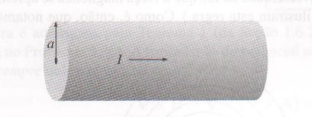
\includegraphics[width=6cm]{Selection_095.jpg} 
\end{figure}

\begin{enumerate}
\item A corrente está uniformemente distribuída sobre a superfície externa do fio.
\item A corrente está distribuída de forma que $J$ é proporcional a $s$, a distância ao eixo.
\end{enumerate}


\textbf{RESOLUÇÃO}

\begin{enumerate}

\item 

Usando a Lei de Ampére, temos:

$$\displaystyle\oint B \cdot dl = B 2\pi s = \mu_0 I_{enc}$$

Temos duas condições:

$$B = 
		\begin{cases}
			0\textrm{,} \quad \quad \quad \textrm{para } s < a \\
			\displaystyle\dfrac{\mu_0 I}{2\pi s}\hat{\phi}\textrm{,} \, \quad \textrm{para } s > a.
		\end{cases}
$$

\item

Pela informação da questão, temos:

$$J = ks$$

Calculando a corrente de $0$ a $a$, temos:

$$I = \displaystyle\int_0^{a} J da = \displaystyle\int_0^{a} ks(2\pi s)ds = \displaystyle\dfrac{2\pi ka^3}{3}$$

Isolando $k$ temos:

$$ k = \displaystyle\dfrac{3I}{2\pi a^3} $$

Dessa forma, podemos escrever:

$$I_{enc} = \displaystyle\int_0^{s} J da = \displaystyle\int_0^{s} ks (2\pi s) ds = \displaystyle\dfrac{2\pi ks^3}{3} = I\displaystyle\dfrac{s^3}{a^3}$$

Podemos concluir dois casos:

$$B = 
		\begin{cases}
			\displaystyle\dfrac{\mu_0 I s^2}{2\pi a^3}\hat{\phi}\textrm{,} \quad \textrm{para } s < a \\
			\\
			\displaystyle\dfrac{\mu_0 I}{2\pi s}\hat{\phi}\textrm{,} \quad \quad \textrm{para } s > a.
		\end{cases}
$$

\end{enumerate}


\item \textbf{Griffiths - Cap. 5 - Problema 5.15.}


Dois solenóides longos e coaxiais transportam, cada um, uma corrente $I$, mas em sentidos opostos, como mostra a figura abaixo. O solenoide interno (de raio $a$) tem $n_1$ voltas por unidade de comprimento, enquanto o externo (de raio $b$) tem $n_2$. Encontre $B$ em cada uma das três regiões:

\begin{figure}[h]	
\centering % para centralizarmos a figura	
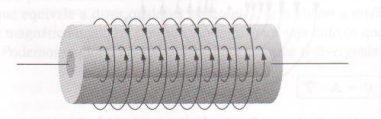
\includegraphics[width=6cm]{Selection_096.jpg} 
\end{figure}

\begin{enumerate}
\item[(i)] dentro do solenoide interno
\item[(ii)] entre eles
\item[(iii)] fora dos dois
\end{enumerate}


\textbf{RESOLUÇÃO}

O cálculo do campo de um solenóide é:


\begin{figure}[h]	
\centering % para centralizarmos a figura	
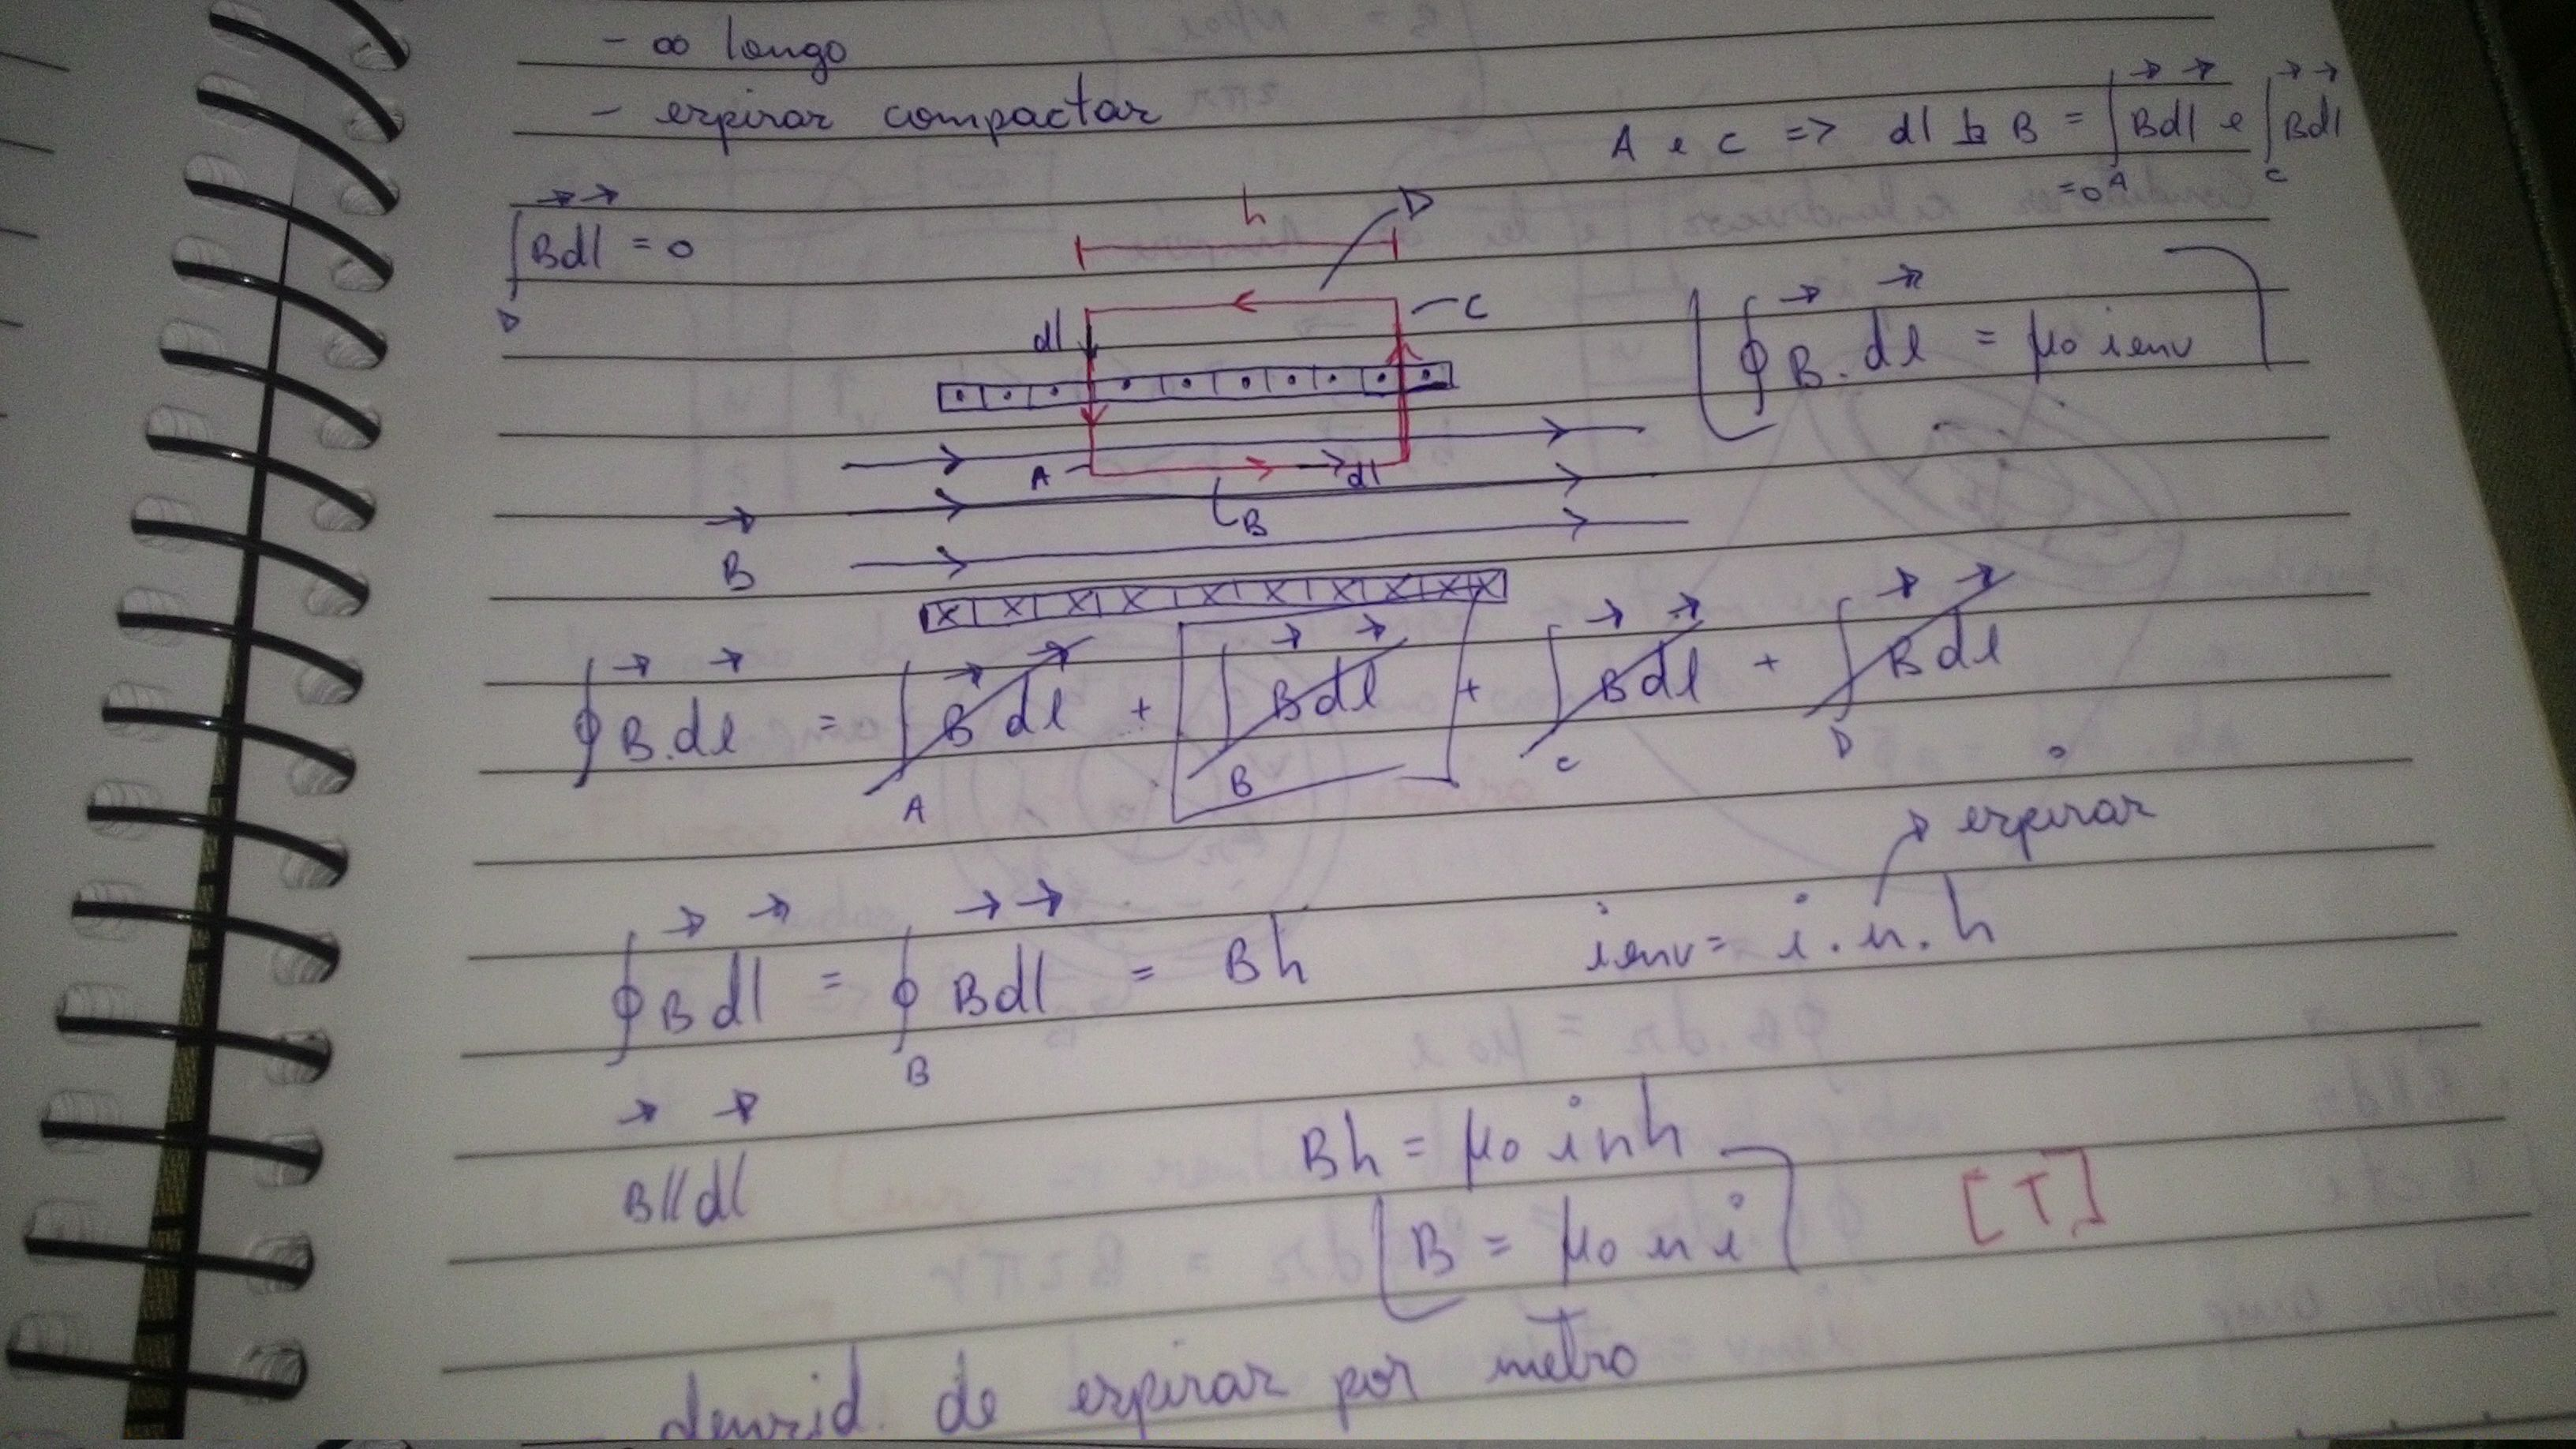
\includegraphics[width=15cm]{P_20180421_220453.jpg} 
\end{figure}

Com os cálculos acima, o campo dentro do solenoide é:

$$B = \mu_0 n I$$

Fora do solenoide o campo é zero. O solenoide mais externo aponta na direção de $-\hat{z}$ sempre que o mais interno aponta para o lado direito $+\hat{z}$. Logo, temos:

\begin{enumerate}
\item[(i)] $B = \mu_0 I (n_1 - n_2) \hat{z}$
\item[(ii)] $B = -\mu_0 I n_2 \hat{z}$
\item[(iii)] $B = 0$
\end{enumerate}


\item \textbf{Griffiths - Cap.5 - Problema 5.18.}

No cálculo de uma corrente encerrada por um circuito amperiano, deve-se, em gral, resolver uma integral com a forma

$$I_{enc} = \displaystyle\int_{S} J \cdot da$$

O problema é que existe uma infinidade de superfícies que compartilham da mesma linha de contorno. Qual delas devemos usar?

\textbf{RESOLUÇÃO}

Não importa qual linha de contorno escolha. A densidade de corrente elétrica $J$ sempre independe da superfície para qualquer simetria. 

\end{enumerate}
	
\end{document}